%!TEX root = ./Body.tex

\chapter{Verfahren} % (fold)
\label{cha:Verfahren}

Wollt ihr hier alle Verfahren haben, oder ein Datei für jeder?\\

blablabla


\section{K-Nearest Neighbor} % (fold)
\label{sec:KNN}
blablabla\\

blablabla
% section Verfahren1 (end)

\section{Random Forests} % (fold)
\label{sec:Forests}
blablabla\\

blablabla
% section Verfahren2 (end)

\section{Neuronale Netze Martin ODER KOMMT NIX?!} % (fold)
\label{sec:NN1}
blablabla\\

blablabla
% section Verfahren3 (end)

\section{Neuronale Netze} % (fold)
\label{sec:NN}
Künstliche Neuronale Netze nehmen das menschliche Gehirn als Vorbild und versuchen so eine Abstraktion von Informationsverarbeitung zu schaffen. Ein neuronales Netz besteht aus mehreren Schichten von Neuronen, die beliebig miteinander verbunden sein können. Zusätzlich zur Netztopologie wird noch eine Aktivierungsfunktion festgelegt, welche das „Feuern“ eines Neurons beschreibt. Der Ablauf bei dem Training des Neuronalen Netzes ist folgendermaßen: zuerst wird eine Netztopologie, eine Anzahl von Neuronen und die Aktivierungsfunktion festgelegt. Die Eingabewerte werden an die Neuronen der ersten Schicht (Eingabeneuronen) angelegt und mittels gewichteter Verbindungen und der Aktivierungsfunktion durch das Netz transportiert. Am Ende liefert die letzte Neuronenschicht (Ausgabeneuronen) einen Wert, welcher mit dem Soll-Wert verglichen wird. Das endgültige Lernen des Neuronalen Netzes ist nun die Anpassung der gewichteten Verbindungen zwischen den Neuronen des Netzes. Allerdings spielt auch die Netztopologie und die Anzahl der Neuronen eine wichtige Rolle. Eine genauere Beschreibung kann z.B. in (James A. Anderson: A simple neural network generating an interactive memory. In: Mathematical Biosciences. 14, 1972, ISSN 0025-5564, S. 197–220. ) nachgeschlagen werden.
Als Implementierung wurde das Framework von Boby Anguelov (http://takinginitiative.net/2008/04/03/basic-neural-network-tutorial-theory/) auf die Aufgabenstellung und die verwendeten Daten angepasst. Dieses Framework bietet ein dreischichtiges FeedForward-Netz und erlaubt eine variable Anzahl an Neuronen pro Schicht. Um die optimale Anzahl an Neuronen zu finden, werden optional sowohl konstruktive als auch destruktive Verfahren angeboten. Wie in Kapitel \ref{cha:Features} erläutert, wurde ein bestimmtes Set an Eingabevektoren ausgewählt und auch die Ausgabeneuronen waren durch die Anzahl der Stellgrößen vorgegeben. Weiterhin kann die Aktivierungsfunktion, sowie die Lernparameter wie Lernrate und Momentumterm angepasst werden. 

Der erste Teil des Trainings befasste sich also damit, die optimale Anzahl an Neuronen für unsere Aufgabenstellung und die Eingangsdaten zu ermitteln. Als desktruktives Verfahren wurde der Optimal Brain Damage Algorithmus (http://yann.lecun.com/exdb/publis/pdf/lecun-90b.pdf ) verwendet, als konstruktives Verfahren die Cascade-Correlation (http://www.cs.iastate.edu/~honavar/fahlman.pdf ). \\

\begin{figure}[!h]
	\centering
	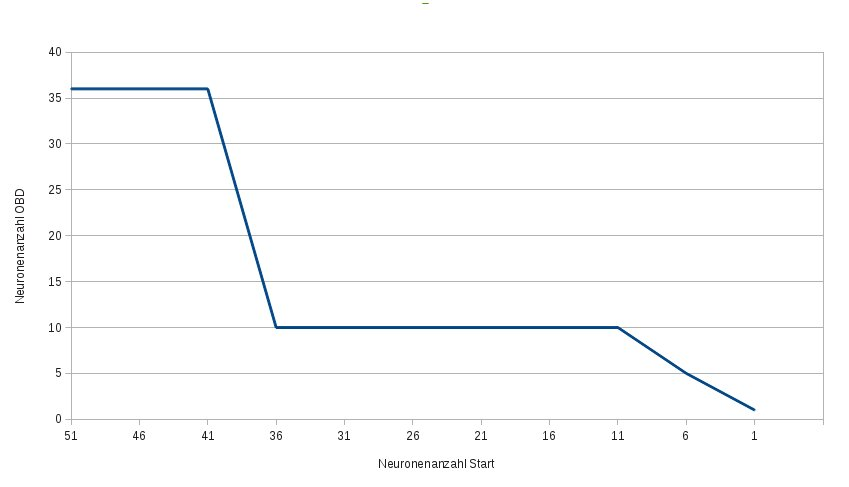
\includegraphics[scale=0.5]{images/nn/a1.jpg} 
	\caption{Ermittelte Neuronenzahl des OBD Algorithmus in Abhängigkeit der Startzahl an Neuronen}
	\label{nnchrisa1}
\end{figure}

Abbildung \ref{nnchrisa1} zeigt die von OBD ermittelte Anzahl an Neuronen abhängig von der Ausgangsneuronenanzahl. Es wird deutlich, dass ein Wert von 10 Neuronen vom Algorithmus als optimal aufgefasst wird; niedrige Werte verschlechtern das Ergebnis deutlich und auch höhere Werte sind bestenfalls gleichwertig. Allerdings benötigt das größere Netz deutlich mehr Zeit und auch eine größere Menge an Trainingsdaten.\\

\begin{figure}[!h]
	\centering
	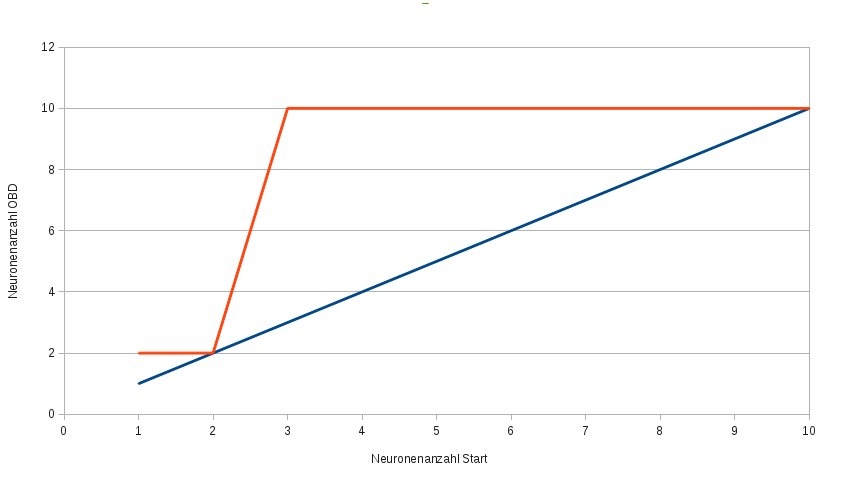
\includegraphics[scale=0.5]{images/nn/a2.jpg} 
	\caption{Ermittelte Neuronenzahl des OBD Algorithmus und des Cascade-Trainings in Abhängigkeit der Startzahl an Neuronen}
	\label{nnchrisa2}
\end{figure}

Abbildung \ref{nnchrisa2} zeigt jeweils die von OBD und dem Cascade Training ermittelte Neuronenzahl in Abhängigkeit vom Startwert für das Intervall zwischen 1 und 10 Neuronen. Das konstruktive Cascade Training lässt die optimale Neuronenzahl sehr deutlich gegen 10 konvergieren, welches vom OBD Algorithmus schon von oben eingegrenzt wurde. Für die weiteren Tests wurde also ein Netz mit 18 Neuronen verwendet, wobei 5 Neuronen als Eingabeneuronen, 10 Neuronen als Hidden-Neuronen, sowie 3 Neuronen als Ausgabeneuronen fungierten.\\

Mit dem festen Netzaufbau wurden nun die Lernrate und der Momentumterm untersucht. Das Training des Neuronalen Netzes wird mittels Gradientenabstieg vorgenommen. Bei diesem Verfahren wird versucht ein globales Minimum in der von den Fehlertermen aufgespannten Hyperebene zu finden. Folgende Probleme können hierbei auftreten:
Lokale Minima: Anstatt des globalen Minimums wird nur ein lokales Minimum gefunden und nicht mehr verlassen. Obwohl eventuell eine bessere Gewichtsverteilung existiert, wird diese nicht mehr gefunden.
Flaches Plateau: Wenn sich der Gradient über eine große Anzahl von Gewichtsanpassungen nicht mehr verändert, dann stagniert das Verfahren. Der Gradient wird so über weitere Schritte so klein, dass keine weitere Erforschung des Raumes mehr erfolgt.
Verlassen guter Minima: Falls ein ausgeprägtes Minimum mit relativ geringer Ausdehnung vorliegt, so kann es übersprungen werden. Also könnte auch so ein globales Minimum übersprungen werden.
Oszillation: Das Verfahren springt von einem Minimum in das nächste, wobei es zwischen beiden Minima hin und her springt. In diesem Fall verändern sich nicht die Beträge der Gradienten, sondern lediglich ihr Vorzeichen.
Eine hohe Lernrate ermöglicht ein schnelles Erforschen der kompletten Hyperebene des Fehlerterms. Flache Plateaus werden schnell durchlaufen und vom Startpunkt weit entfernte Minima werden schnell erreicht. Allerdings steigt auch die Gefahr gute (bzw. globale) Minima zu überspringen oder zwischen gefundenen Minima zu oszillieren. Bei einer Lernrate von 0.9 trat genau dies bei den Trainingsdaten auf. Das Training benötigte zwar nur eine kurze Zeit (eine Minute), allerdings zeigte sich dann eine komplette Oszillation.
Eine niedrige Lernrate kann komplexe Lerndaten, sowie eine große Datendichte besser bewältigen, ist weniger anfällig für Oszillation und für das Überspringen von Minima. Allerdings erhöht sich dadurch die Trainingszeit und Plateaus, sowie lokale Minima können nicht mehr überwunden werden. Dies zeigte eine Lernrate von 0.01 deutlich: das Training benötigte mehr als 12 Stunden und es wurde das „erstbeste“ Minimum nicht mehr verlassen.
Um die Nachteile einer niedrigen Lernrate auszugleichen, kann man ein Momentum einführen. Dieser Trägheitsterm berücksichtigt zusätzlich zur aktuellen Änderung des Gradienten auch die vorausgegangene Änderung. Hiermit wird ein schnelles überqueren von Plateaus ermöglicht.
Als endgültige Parameter wurden eine Lernrate von 0.1 und ein Momentum von 0.9 gewählt.\\

Die letzte Stellschraube des Lernverfahrens war die erlaubte Varianz im Vergleich der Soll- und Istwerte der Ausgabeneuronen. Da hier keine klassische Klassifikation, also ein binärer Vergleich, stattfand, sondern eine kontinuierliche Funktion gelernt werden sollte, muss dem Lernalgorithmen ein gewisser Spielraum gegeben werden. Weiterhin ist dieser Schritt damit motiviert, dass der Fahrsimulator nur Werte mit bestimmter Genauigkeit annahm, z.B. die Gaspedalstellung in Tausendstel-schritten. Eine hohe Varianz erleichtert natürlich das grobe Einlernen dieser Funktion, wobei eine niedrige Varianz die Funktion besser beschreiben sollte.\\

\begin{figure}[!h]
	\centering
	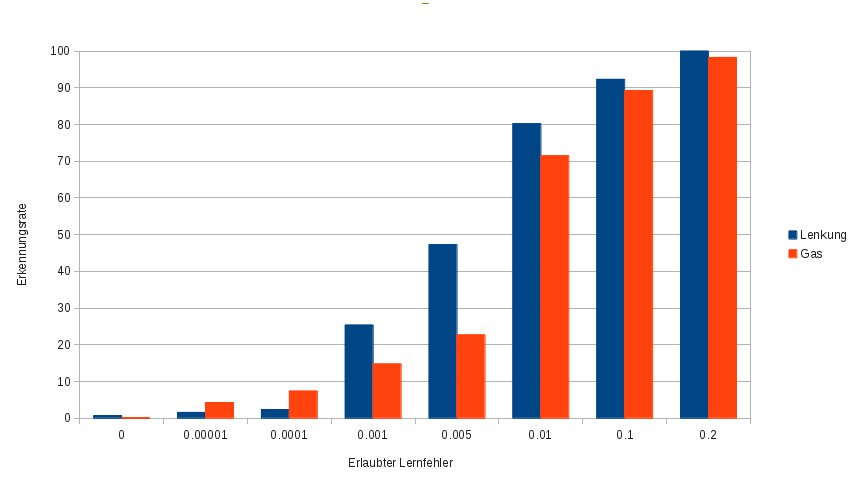
\includegraphics[scale=0.55]{images/nn/a3.jpg} 
	\caption{Erkennungsrate der Stellgrößen Gaspedalstellung und Lenkwinkel in Abhängigkeit der zugelassenen Fehlervarianz}
	\label{nnchrisa3}
\end{figure}

Abbildung \ref{nnchrisa3} zeigt die Erkennungsrate von Gaspedalstellung und Lenkwinkel in Abhängigkeit des erlaubten Lernfehlers. Eine allgemeine Aussage war hier nicht möglich, da in der Praxis die Gaspedalstellung mit wenig Fehlervarianz und somit niedriger Erkennungsrate, jedoch beim Lenkwinkel eine relativ hohe Fehlervarianz mit hoher Erkennungsrate besser funktionierte. 
% section Verfahren4 (end)

\section{Support Vector Regression} % (fold)
\label{sec:SVR}
blablabla\\

blablabla
% section Verfahren5 (end)


% chapter Verfahren (end)